% Kapitel 2 mit den entsprechenden Unterkapiteln
% Die Unterkapitel können auch in separaten Dateien stehen,
% die dann mit dem \include-Befehl eingebunden werden.
%-------------------------------------------------------------------------------
\chapter{Analyse der Produktfunktionen}

%Die Kapitel müssen mit Inhalt gefüllt werden!. Eine Bereiche habe ich beuwsst schon bei der Verteildung der Diagramme zusammengefasst 
%In diesen Bereichen möchte ich euch bitten die jeweiligen Unterpunkte kurz mit den Oberpunkten zu vergleichen und zu argumentieren 
%warum es sich um triviale Spezialfälle handelt die keiner näheren beschreibung bedürfen
%
% Ich hab mal immer davon geschrieben welche Bereich von wem gemacht werden

\section{Analyse der Funktionalität /F100/: Spezifikation einlesen}
Das Einlesen einer Spezifikation aus einem vom Nutzer angegebenen Dateipfad
gliedert sich in mehrere Teilfunktionalitäten. Zunächst muss der Anwender den
Dateipfad auswählen. Dafür sollte ein Datei-Dialog zum Einsatz kommen.
Danach muss die ausgewählte Datei geöffnet, geprüft und geparst werden. Für
diese Aufgaben bietet sich eine spezialisierte Komponente an, um alle
Eigenheiten des Dateiformates von der Oberfläche und dem Simulator abzukapseln.
Der ausgelesene Datensatz wird nun zum Starten einer neuen Simulation verwendet,
dafür muss eine eventuell laufende Simulation beendet werden. Es bietet sich
an, diese Funktionen als Schnittstelle zu kapseln und die konkrete Implementierung
der Simulator-Komponente zu überlassen.

\begin{figure}
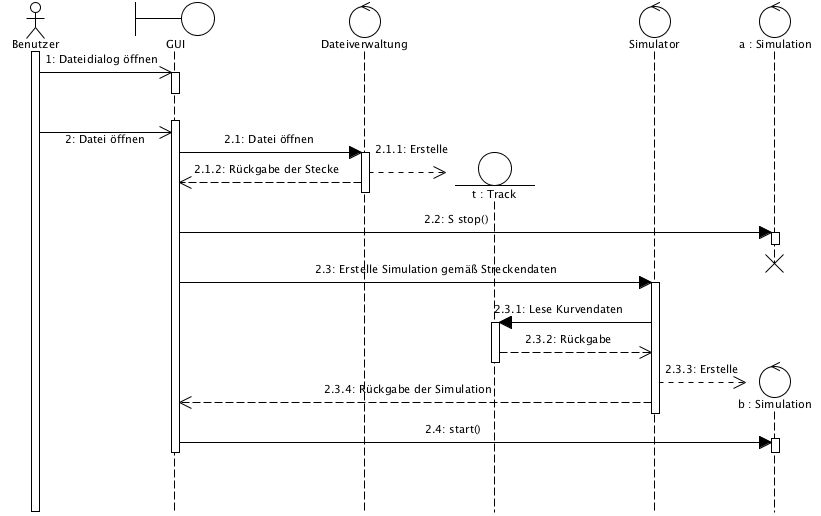
\includegraphics[width=\linewidth]{bilder/spezifikation_einlesen}
\caption{Sequenzdiagramm für \textit{Spezifikation einlesen}}
\end{figure}

%Christian/Matthias

%kann man dies ggf Q40 zuordnen?
\section{Analyse von Funktionalität :  Renderloop}
Da es sich um ein System handelt, in dem eine ständige Berechnung (Loop) zur Laufzeit notwendig wird, einerseits durch die 3D-Anzeige, die eine ständige Aktualisierung erwartet und andererseits durch
die Simulation an sich, ist es sinnig diesen Vorgang ebenfalls näher zu beleuchten.

\begin{figure}
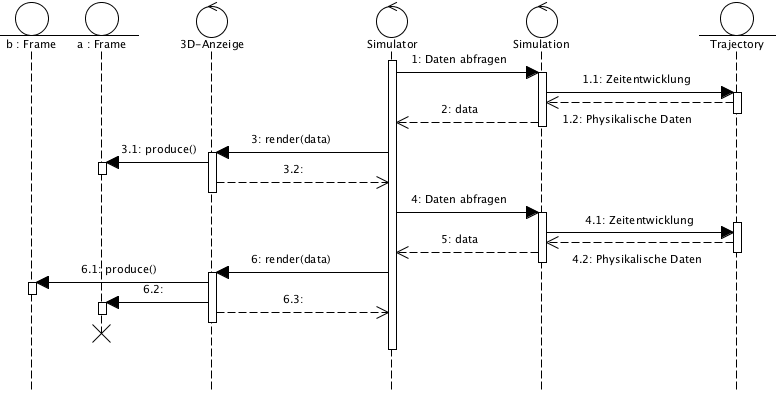
\includegraphics[width=\linewidth]{bilder/render_loop}
\caption{Sequenzdiagramm für \textit{Renderloop}}
%\label{labelname}
\end{figure}

Der Simulator initiiert einen Simulationsschritt indem ein neuer Simulationsschritt bei der Simulation angefordert  wird. Die erhalten Daten werden dann zur 3D-Anzeige weitergereicht und werden dort visualisiert.

%Simon:
\section{Analyse von Funktionalität /F200/ :  Starten/Stoppen der Simulation}
Der Anwender kann über die GUI die Simulation starten. Dabei wird die Information an den Simulator weitergeleitet, der das 3D Bild anzeigt, die 2D Statusanzeige einblendet, die Bahnberechnung startet und die Aufzeichnung startet. 
Der Anwender kann außerdem über die GUI die Simulation stoppen. Dabei wird die Information ebenfalls an den Simulator weitergeleitet, der dann alles wieder schließt und die Aufzeichnung speichert.

\begin{figure}
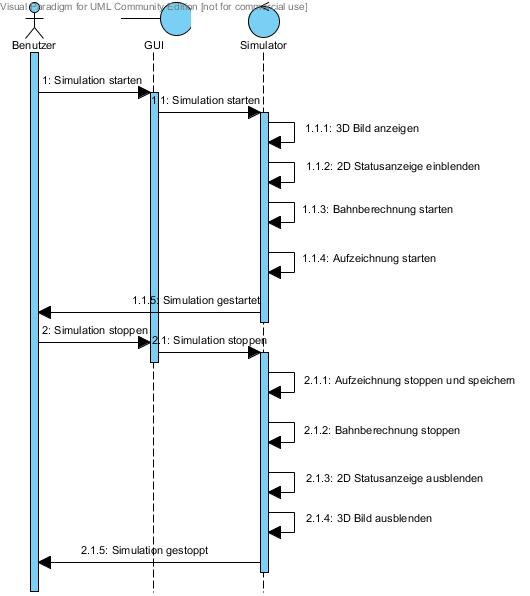
\includegraphics[width=\linewidth]{bilder/Simulator_Starten_Stoppen}
\caption{Sequenzdiagramm für das \textit{Starten und Stoppen der Simulation}}
%\label{labelname}
\end{figure}

%Robin
\section{Analyse von Funktionalität /F300/ :  Pausieren der Simulation}
Der Anwender hat während der Simulation die Möglichkeit diese anzuhalten und sie später fortzusetzen, ohne dass die Pausierung Auswirkungen auf das Simulationsergebnis hat.

\begin{figure}
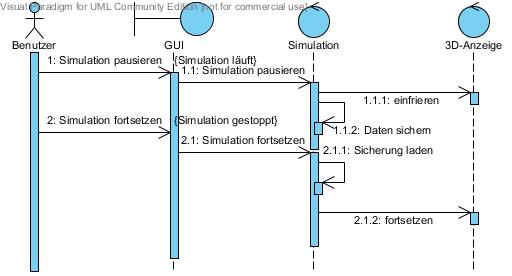
\includegraphics[width=\linewidth]{bilder/Pausieren.jpg}
\caption{Sequenzdiagramm für \textit{Pausieren der Simulation}}
%\label{labelname}
\end{figure}

%Daniel
\section{Analyse von Funktionalität /F400o/ :  Video aufzeichnen}
Der Anwender kann über die GUI die Eingabe tätigen, ein Video aufzeichnen zu wollen, sofern nicht gerade eine Aufnahme läuft. Die GUI gibt diese Anweisung an die 3D-Anzeige weiter, die nun mit der
Videoaufnahme beginnt. Dies geschieht so lange, bis der Anwender die Videoaufzeichnung stoppt. In diesem Fall wird die Aufzeichnung angehalten und die Videodatei wird gespeichert.


\begin{figure}
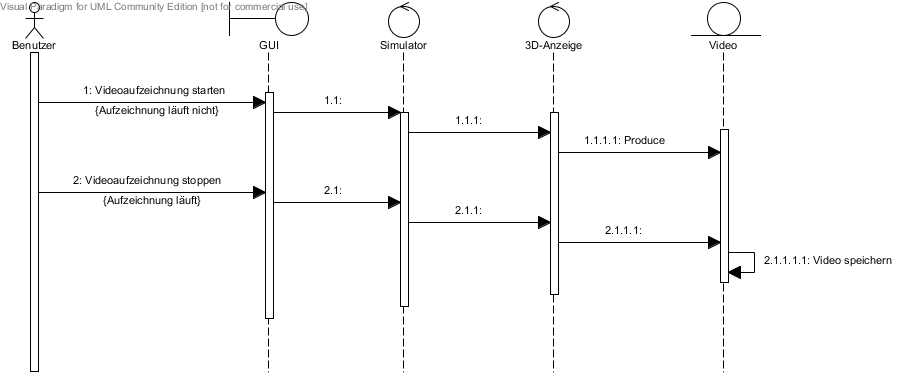
\includegraphics[width=\linewidth]{bilder/Video_aufzeichnen}
\caption{Sequenzdiagramm für \textit{Video aufzeichnen}}
%\label{labelname}
\end{figure}

%Matthias/Christian
\section{Analyse von Funktionalität /F500/ :  Einstellungen ändern}
\subsection{Analyse von Funktionalität /F510o/ :  Physikalische Parameter anpassen}
Der Benutzer kann auf der GUI die physikalischen Parameter anpassen. Dabei wird allerdings die Simulation gestoppt, weil es nicht wissenschaftlich wertvoll ist, während der Fahrt physikalische Parameter zu ändern. Der Benutzer muss deshalb die Simulation mit anderen Parametern neu starten.

\begin{figure}
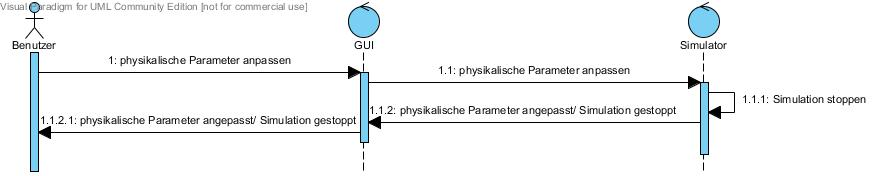
\includegraphics[width=\linewidth]{bilder/Physikalische_Parameter_anpassen.jpg}
\caption{Sequenzdiagramm für \textit{Physikalische Paramter anpassen}}
%\label{labelname}
\end{figure}

\subsubsection{Analyse von Funktionalität /F511o/ :  Gravitation anpassen}
Der Benutzer kann bei bedarf die Gravitation verändern, indem er auf der GUI die Einstellung vornimmt. Dabei wird, wie bei allen Änderungen der Physik, die Simulation gestoppt.
\subsubsection{Analyse von Funktionalität /F512o/ :  Wagenmasse anpassen}
Der Benutzer kann bei bedarf die Wagenmasse verändern, indem er auf der GUI die Einstellung vornimmt. Dabei wird, wie bei allen Änderungen der Physik, die Simulation gestoppt.
%Matthias
\subsection{Analyse von Funktionalität /F520/ :  Simulationsparameter ändern}
Die Veränderung von Parametern die die Simulation direkt betreffen fallen unter diese Oberklasse. Die einzelnen Unterpunkte werden in den 2 folgenden Kapiteln erläutert. Im wesentlichen Fallen hier 
auch einfache Veränderungen an, die als atomistisch und somit unkritisch anzusehen sind. In der Folge werden diese Use-Cases nicht extra in Sequenzdiagrammen abgebildet.
\subsubsection{Analyse von Funktionalität /F521o/ :  Dekorative Umgebung anpassen}
Da diese Aktion in den Datenbestand des 3D-Kontext eingreift, gibt es einen interessanten Fall, in dem das direkte Setzen der Deko nicht möglich ist. 
Der Nutzer fordert die Veränderung der Deko über die GUI an (3). Kurz zuvor wurde aber das Rendern eine Frames(1) angefordert. 
In der Folge muss die GUI warten bis der Simulator das Rendern des Frames abgeschlossen hat(2) und kann erst dann seine Änderungen melden (3.2) die an die 3D-Anzeige weitergereicht werden(3.2.1) und dort angewendet werden.

\begin{figure}
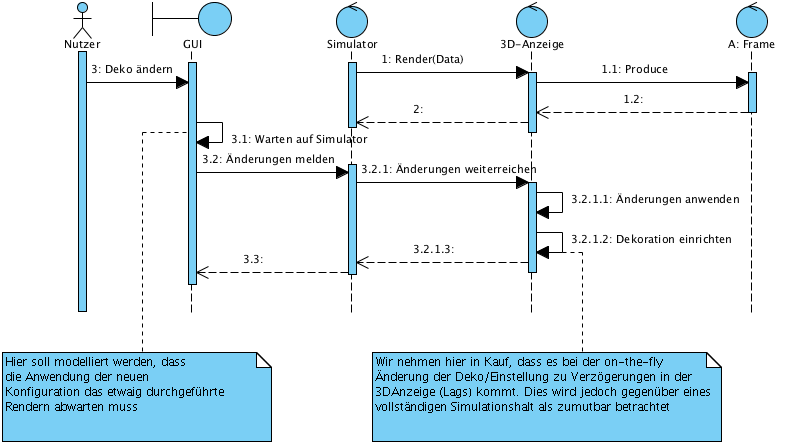
\includegraphics[width=\linewidth]{bilder/change_graphic_deko}
\caption{Sequenzdiagramm für \textit{Dekorative Umgebung anpassen}}
%\label{labelname}
\end{figure}
Es wird hier in Kauf genommen, dass die Simulation für eine spürbare Zeit unterbrochen wird, um die Deko zu laden. Dies wird als zumutbar angenommen, um undefinierte Zustände zu verhindern. 
Außerdem wird erwartet, dass die Funktionalität selten während der laufenden Simulation, sondern vor dem Start genutzt, wird wo auch Wartezeiten akzeptabel sind.
Auch ist die notwendigkeit des Wartens der GUI auf den Simulator unkritisch, da die Berechnung eines Frames üblicherweise 20 mal pro Sekunde erfolgt, sodass die resultierende Verzögerung minimal ist.

\subsubsection{Analyse von Funktionalität /F522o/ :  Simulationszeit anpassen}
Die Simulationsgeschwindigkeit wird aufgrund der Implementierung eines numerischen Lösungsverfahrens für die Berechnung der Daten ein diskreter Zeitschritt sein. Dieser Wert kann direkt und entsprechend
den Anforderungen des Nutzers gesetzt werden. Das einfache Durchreichen über die GUI an den Simulator wird nicht in einem zusätzlichen Sequenzdiagramm dargestellt.
%Matthias
\subsection{Analyse von Funktionalität /F530/ :  Grafische Einstellungen ändern}
Die Anpassung der grafischen Einstellung bezieht sich hier zunächst allgemein auf grafische Einstellungen. Besonders interessant ist dabei jedoch der Fall der Veränderung von Einstellungen, die 
die 3D-Anzeige betreffen. 

\begin{figure}
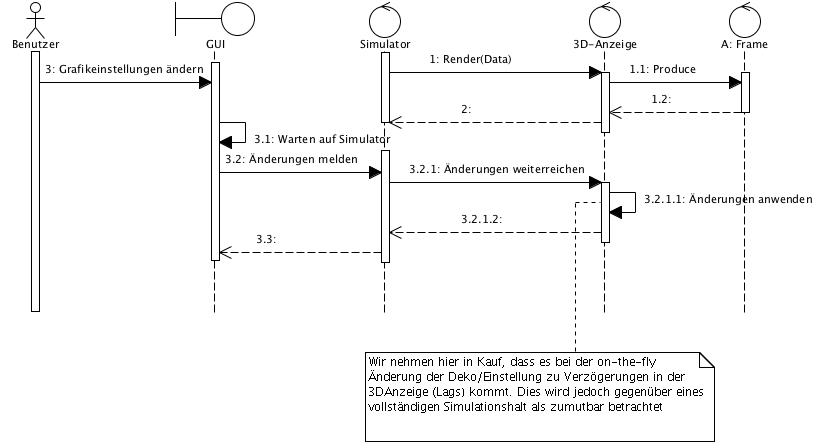
\includegraphics[width=\linewidth]{bilder/change_graphic_config}
\caption{Sequenzdiagramm für \textit{Graphische Einstellungen ändern}}
%\label{labelname}
\end{figure}
Fordert der Nutzer die Veränderung von Einstellungen aus dem 3D-Kontext an (3), so besteht die Möglichkeit, dass zum gleichen Zeitpunkt ein Frame, initiiert durch den Simulator (1), gerendert wird. 
Die GUI (hier für den 2D-Anteil) wird die Anfrage des Benutzer an den Simulator weiterreichen (3.2) sobald der Renderprozess abgeschlossen ist (2). Die Änderungen an den Einstellungen können dann weitergemeldet (3.2.1) und angewandt (3.2.1.1) werden.

Bei diesem Vorgehen wird in Kauf genommen, dass es für das Frame, welches auf die Einstellungsänderung folgt, zu einer Verzögerung in der Darstellung kommt. Dies muss jedoch als zumutbar erachtet werden, da eine Zeitdauer im Millisekundenbereich zu erwartet ist. Die Alternativen beinhalten wesentlich störendere Artefakte oder aber das grundsätzliche Anhalten der Simulation nach Änderungen an den Einstellungen.

%Daniel
\subsection{Analyse von Funktionalität /F531/ :   Neuanordnung (Interface)}
Der Anwender hat die Möglichkeit, die Elemente der GUI nach seinen eigenen Bedürfnissen anzuordnen. Dafür ändert der Nutzer Einstellungen in der GUI.
\begin{figure}
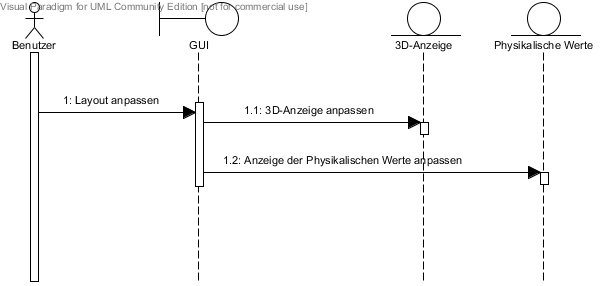
\includegraphics[width=\linewidth]{bilder/Interface_Neuanordnung}
\caption{Sequenzdiagramm für \textit{Neuanordnung (Interface)}}
%\label{labelname}
\end{figure}
%Simon
\subsubsection{Analyse von Funktionalität /F532/ :  Ein-/Ausblenden von Beschleunigungsdaten}
Der Anwender hat die Möglichkeit, sich die Beschleunigungsdaten anzeigen zu lassen. Dabei werden die Daten berechnet und an die GUI übergeben, wo die Beschleunigung dann anzeigt wird. Zusätzlich hat der Anwender die Möglichkeit, die Beschleunigungsdaten wieder auszublenden.
\begin{figure}
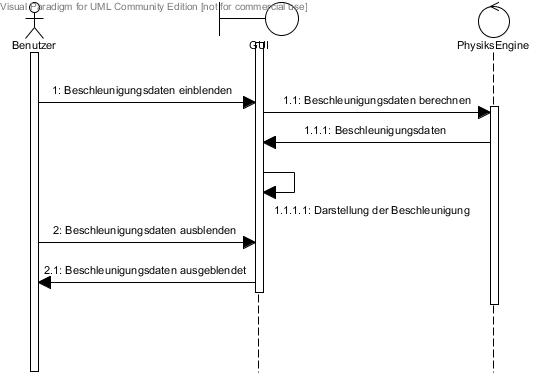
\includegraphics[width=\linewidth]{bilder/Simulator_Beschleunigung}
\caption{Sequenzdiagramm für \textit{Ein-/Ausblenden von Beschleunigunsdaten}}
%\label{labelname}
\end{figure}
%Robin
\subsubsection{Analyse von Funktionalität /F533o/ :  Kameraperspektive ändern}
Während der Simulation kann der Anwender die Perspektive der Kamera ändern, ohne dass dabei die Simulation unterbrochen wird. Um einen unterbrechungsfreien Ablauf zu erreichen, errechnet die Simulation zum nächstmöglichen Zeitpunkt die gewählte Kameraeinstellung und stellt sie ab diesem Zeitpunkt dar. 
\begin{figure}
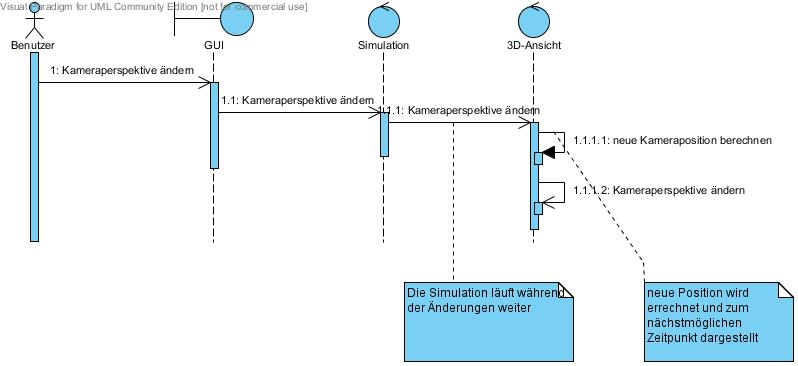
\includegraphics[width=\linewidth]{bilder/Kameraperspektive.jpg}
\caption{Änderung der Kameraperspektive}
\label{Kameraperspektive}
\end{figure}
%Konstantin
\section{Analyse von Funktionalität /F1000/ :  Warnung vor hoher Beschleunigung}
%zweiter Versuch
Falls während der Simulation eine zu hohe, d.h. für Menschen ungesunde oder tötliche Beschleunigung auftritt, wird eine entsprechende Warnung in der GUI ausgegeben.
\begin{figure}
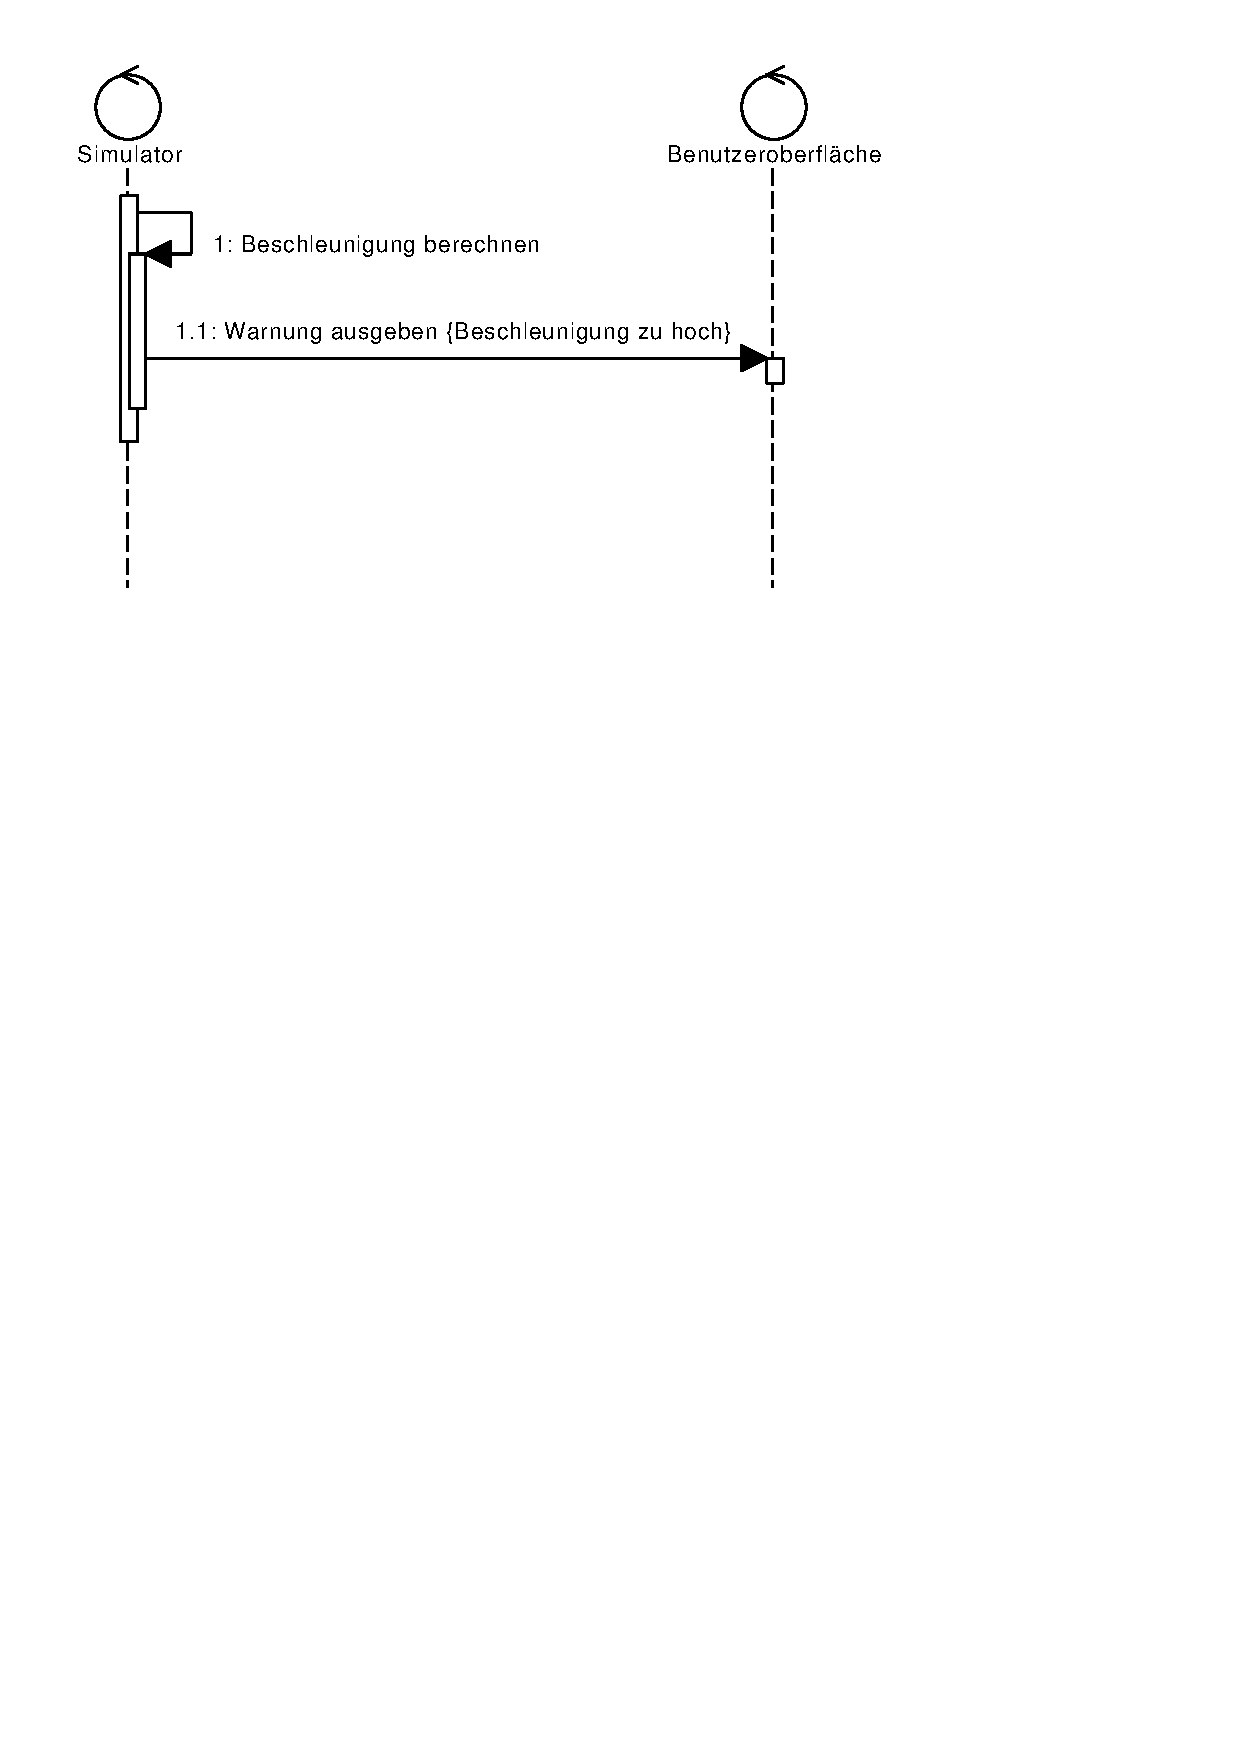
\includegraphics[width=\linewidth]{bilder/Warnung_Beschleunigung}
\caption{Warnung vor zu hoher Beschleunigung}
%\label{labelname}
\end{figure}
%Marco:
\section{Analyse von Funktionalität /F1100/ :  Erkennung von Veränderungen an der Ursprungsdatei}
